% !TEX root = ../notes_unsupervisedlearning.tex
% Chapter 1: Foundations
%%%%%%%%%%%%%%%%%%%%%%%%%%%%%%%%%%%%%%%%%%%%%%%%%%%%%%%%%%%%%%%%%%%%%%

% POST IMPROVEMENTS 2026:
% 1. Cosine alternatives for similar feature space
% 2. Cosine similarity for semantic similarity in NLP - also in embeddings?

% Run the audio file for all lecture notes, after you updated them? Or make this a monthly script that runs only if something changed? 

% THIS NEXT POINT WILL BE THE MAIN CONTRIBUTION OF THE SECOND YEAR IN ALL LECTURES.
% Make them watch the calculations afterwards or maybe even beforehand? 
% 3. Do the calculations on paper, make a recording of it, and link to it in the margin note. Share it with students (flipped classroom style).

% 4. Repurpose the plots from the jupyter notebooks in the script. e.g. showing clusterings for dense point clouds.
% 5. Add a full page on elbow methods, if not here then in the next block Kneedle (Satopaa et al., 2011) — the standard algorithmic elbow finder. Normalise both axes to $[0,1]$, compute the difference between the curve and the diagonal connecting endpoints, find the maximum. Works on any monotone-curving curve. Implementation: kneed Python package.
% Maximum curvature — the elbow is where the curve bends most sharply: $\kappa(k) = \frac{|y''|}{(1 + y'^2)^{3/2}}$ is maximal. Analytical when you have a fitted model of $y(k)$, numerical otherwise.
% L-method — connect first and last points with a straight line, pick the $k$ whose perpendicular distance from that line is largest. Equivalent to Kneedle in spirit.



\index{Foundations}\index{Distance Metrics}\index{similarity}\index{distance}
\chapter{Similarity and Distance}
\newthought{Enter the Feature Space}

% ==============================================================================================
% BLOCK 1: INTRODUCTION
% ==============================================================================================

\section{The Why}\index{unsupervised learning}

In supervised learning\index{supervised learning}\cite{DeepLearningBook}, the learning process relies on data samples $x$ paired with their ground truth labels $\tilde{y}$, which allows a
model $\theta$ to learn a mapping,

\marginnote{\newthought{On the concept of truth}, $\tilde{y}$, while being called ground truth, 
is often an approximation of the true label $y$. 
It may come from human annotation, measurements, or other sources.}

\begin{align*}
    \theta(x) &= \hat{y},\\
                &\approx \tilde{y}.
\end{align*}


The presence of labels provides a clear signal for learning, as it allows optimization of a loss function that measures the discrepancy between predictions and true labels.
The loss then guides the learning process, enabling the model to adjust its parameters along the gradient to minimize this discrepancy:

\begin{align*}
    \theta &\leftarrow \theta - \eta \nabla_\theta \mathcal{L}(\hat{y}, \tilde{y}).
\end{align*}

\newthought{Facing the absence of labels}, we are left with only the data samples\cite{DIKWpyramid} $x$ and no explicit signal to guide learning.
The methods we will explore in this course are designed to discover and leverage the inherent structure and patterns\cite{Bishop2006} in the data itself, 
without relying on external supervision, thus mostly referred to as unsupervised learning.\index{pattern recognition}

\marginnote{\newthought{Knowledge Pyramid}\\
Data ($1$) raw signal\\
$\to$ Information (\textit{banana}) endowed with meaning \\
$\to$ Knowledge ($\neq$ \textit{coffee}) structured and contextualized information \\
$\to$ Wisdom or \textit{knowing and appreciating the Why}.}

\newthought{In a first step} this requires us to,
\begin{itemize}
    \item define what we mean by pattern in the context of data.
    \item understand the geometry of data, which includes concepts of distance, similarity, and neighborhood.
    \item learn how to engineer data representations that make pattern more accessible.
\end{itemize}

\newthought{The fundamental question} in unsupervised learning is to find pattern, represent it, and utilize it.







\subsection{Hands On Experience}

\newthought{Consider} six data points in two dimensions. Which points seem to belong together? 
Why do you think that? How many groups do you see? To which group would you assign new points?
Draw areas around each group. 

\begin{figure}
\centering
\begin{tikzpicture}[scale=1]
    \begin{axis}[
        xmin=0, xmax=10,
        ymin=0, ymax=10,
        width=0.5*\textwidth,
        height=0.5*\textwidth,
        axis line style={draw=none}, 
        tick style={black, thick},
        xtick={1,2,3,6,8},
        ytick={1,2,3,7,8,9},
        xticklabel style={font=\small},
        yticklabel style={font=\small},
        tick align=outside,
        tick pos=left, % Only show ticks on left and bottom
    ]
    \addplot[only marks, mark=*, mark size=2pt, black] coordinates {
        (1,2) (2,3) (3,1)
        (6,8) (8,7) (8,9)
    };
    \end{axis}
\end{tikzpicture}
\caption{Six points in 2D. Can you see the two clusters? Or are there six? Or maybe one?}
\label{fig:six_points}
\end{figure}



\newthought{Without labels}, pattern are ambiguous. With just a single additional point, the pattern can change drastically.
Where does the new point belong? Does it belong to the first cluster, the second, or does it form its own cluster?
Does this new point change the pattern of the original six points? How would you draw areas around the clusters now? 
How did that change your assumptions of the first pattern? 

\begin{figure}
\centering
\begin{tikzpicture}[scale=1]
    \begin{axis}[
        xmin=0, xmax=10,
        ymin=0, ymax=10,
        width=0.5*\textwidth,
        height=0.5*\textwidth,
        axis line style={draw=none}, 
        tick style={black, thick},
        xtick={1,2,3,6,8},
        ytick={1,2,3,7,8,9},
        xticklabel style={font=\small},
        yticklabel style={font=\small},
        tick align=outside,
        tick pos=left, % Only show ticks on left and bottom
    ]
    \addplot[only marks, mark=*, mark size=2pt, black] coordinates {
        (1,2) (2,3) (3,1) (3,7)
        (6,8) (8,7) (8,9)
    };
    \end{axis}
\end{tikzpicture}
\caption{Seven points in 2D. The point at $(3, 7)$ creates ambiguity. Is it part of the first cluster, the second, or its own cluster?}
\label{fig:seven_points}
\end{figure}

\marginnote{\newthought{Pareidoly} is the tendency to perceive meaningful patterns in random data. Such as animals in clouds.}
\newthought{Humans are remarably good at finding pattern in data}, even with very little information, and even if it is completely off.
It is a fundamental part of our cognition, and it is what allows us to make sense of the world. However, it also motivates the need
for methods to quantify and formalize pattern. On that note it is also good practice to start with a hypothesis of what you expect to find in the data, and then test that hypothesis with the data, 
rather than just looking for any pattern that may emerge. And on a short managerial note, if the knowledge you will gain will not 
make you take action, then don't waste your time measuring it in the first place.


\newthought{The Learning Objectives} of this lecture are that you will be able to:
\begin{itemize}
    \item Understand the key role of distance and similarity in unsupervised learning and pattern recognition.
    \item Compute and interpret common distance metrics (Euclidean, Manhattan, Cosine, Mahalanobis).
    \item Apply appropriate normalization and scaling strategies and understand why they are necessary.
\end{itemize}





% ==============================================================================================
% BLOCK 2: MAIN THEORY
% ==============================================================================================

\newpage


\section{Distance and Similarity}\index{distance metric}\index{feature space}


\newthought{Quite intuitively}, you already connected points and formed groups in terms of a similarity which was 
based on the closeness between data points. This concept will carry you very far.\\

\newthought{A distance function}\index{distance function} $d: X \times X \to \mathbb{R}_{\geq 0}$, which means taking two samples out of the set $X$,
mapping them to a non-negative real number, must satisfy:\index{metric properties}
\begin{align}
    &\text{Non-negativity:} && d(x, y) \geq 0 \label{eq:nonnegativity} \\
    &\text{Identity:}       && d(x, y) = 0 \iff x = y \label{eq:identity} \\
    &\text{Symmetry:}       && d(x, y) = d(y, x) \label{eq:symmetry} \\
    &\text{Triangle inequality:} && d(x, z) \leq d(x, y) + d(y, z) \label{eq:triangle}
\end{align}

\newthought{Euclidean Distance}\index{Euclidean distance}\index{L2 distance} is probably the most familiar distance metric, measuring the straight-line distance between two points in space.


\begin{figure}
\centering
\begin{tikzpicture}[scale=1]
    \begin{axis}[
        xmin=0, xmax=10,
        ymin=0, ymax=10,
        width=0.5*\textwidth,
        height=0.5*\textwidth,
        axis line style={draw=none}, 
        tick style={black, thick},
        xtick={1,2,3,6,8},
        ytick={1,2,3,7,8,9},
        xticklabel style={font=\small},
        yticklabel style={font=\small},
        tick align=outside,
        tick pos=left, % Only show ticks on left and bottom
    ]
    \addplot[only marks, mark=*, mark size=2pt, black] coordinates {
        (3,1)
        (6,8) 
    };
    
    \addplot[only marks, mark=*, mark size=2pt, black!30] coordinates {
        (1,2) (2,3)
        (8,7) (8,9)
    };
    % Draw a line between (3,1) and (6,8)
    \addplot[thin, black] coordinates {(3,1) (6,8)};
    \end{axis}
\end{tikzpicture}
\caption{Euclidean distance between points (3,1) and (6,8).}
\label{fig:six_points_euclidean}
\end{figure}


And it was probably the one you implicitly used to connect the points in the previous exercise. It is defined as:

\marginnote{Calculating the Euclidean distance between points $A=(3,1)$ and $B=(6,8)$:
\begin{align*}
    d(A, B) &= \sqrt{(6-3)^2 + (8-1)^2} \\
    &= \sqrt{9 + 49} \\
    &= \sqrt{58} 
    &\approx 7.62
\end{align*}}
\begin{align*}
    d_{\text{Euclidean}}(x, y) &= \sqrt{\sum_{i=1}^{n} (x_i - y_i)^2} \\
    &= \|x - y\|_2
\end{align*}

\marginnote{\newthought{Features} can be thought of as dimensions in a vector space. Each data point is a vector in this space.}

\newthought{Euclidean distance} assumes all dimensions are equally important and measured in the same units.\index{geometric assumptions} It also assumes a continuous, smooth space.
It is trivial to think of scenarios where these assumptions do not hold, such as when features have different scales (e.g. age vs. income)
or when the features are not linearly related or not equaly important (e.g. size vs. IQ). And then there are the cases where the
units are ambiguous for the task like distances on maps.





\vspace{2.5em}
\newthought{Manhattan Distance}\index{Manhattan distance}\index{L1 distance} is also called $L_1$ distance or taxicab distance. Instead of measuring the euclidean distance, it measures the axis-aligned path along grid lines:



\begin{figure}
\centering
\begin{tikzpicture}[scale=1]
    \begin{axis}[
        xmin=0, xmax=10,
        ymin=0, ymax=10,
        width=0.5*\textwidth,
        height=0.5*\textwidth,
        axis line style={draw=none},
        tick style={black, thick},
        xtick={1,2,3,6,8},
        ytick={1,2,3,7,8,9},
        xticklabel style={font=\small},
        yticklabel style={font=\small},
        tick align=outside,
        tick pos=left,
    ]
    \addplot[only marks, mark=*, mark size=2pt, black] coordinates {
        (3,1)
        (6,8)
    };
    \addplot[only marks, mark=*, mark size=2pt, black!30] coordinates {
        (1,2) (2,3)
        (8,7) (8,9)
    };
    % Draw Manhattan path: (3,1) to (3,8), then (3,8) to (6,8)
    \addplot[thin, black] coordinates {(3,1) (3,8) (6,8)};
    \end{axis}
\end{tikzpicture}
\caption{Manhattan (taxicab) distance between points (3,1) and (6,8): path follows grid lines.}
\label{fig:six_points_manhattan}
\end{figure}
\begin{marginfigure}
    \centering
    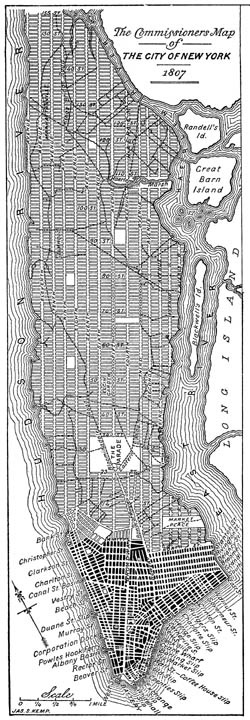
\includegraphics[width=0.75\marginparwidth, trim=0 0 0 360bp, clip]{./figures/Grid_1811.jpg}
    \caption{Grid, 1811 (public domain) see Bridgeman Art Library v. Corel Corp.}
\end{marginfigure}
\marginnote{Calculating the Manhattan distance between points $A=(3,1)$ and $B=(6,8)$:
\begin{align*}
    d_M(A, B) &= |6-3| + |8-1| \\
    &= 3 + 7 \\
    &= 10
\end{align*}}
\begin{align*}
    d_{\text{Manhattan}}(x, y) &= \sum_{i=1}^{n} |x_i - y_i| \\
    &= \|x - y\|_1
\end{align*}

\newthought{Especially useful} when movement is constrained to axes, such as for city blocks like the ones in Manhattan, pixel grids, or when you want robustness to outliers in individual dimensions.


\vspace{2.5em}
\newthought{Cosine Similarity}\index{Cosine similarity} measures the angle between two vectors,
ignoring their magnitude. It is especially useful when the correlation of the features of the data matters more than its absolute values.


\begin{figure}
\centering
\begin{tikzpicture}[scale=1]
    \begin{axis}[
        xmin=0, xmax=10,
        ymin=0, ymax=10,
        width=0.5*\textwidth,
        height=0.5*\textwidth,
        axis line style={draw=none},
        tick style={black, thick},
        xtick={0, 1,2,3,6,8},
        ytick={0, 1,2,3,7,8,9},
        xticklabel style={font=\small},
        yticklabel style={font=\small},
        tick align=outside,
        tick pos=left,
    ]
    \addplot[only marks, mark=*, mark size=2pt, black] coordinates {
        (3,1)
        (6,8)
    };
    \addplot[only marks, mark=*, mark size=2pt, black!30] coordinates {
        (1,2) (2,3)
        (8,7) (8,9)
    };
    % Draw vectors from origin to A and B
    \addplot[->, thin, black] coordinates {(0,0) (3,1)};
    \addplot[->, thin, black] coordinates {(0,0) (6,8)};
    % Angle arc from 18.4 deg to 53.1 deg
    \addplot[thin, black, domain=18.4:53.1, samples=30] ({2*cos(x)}, {2*sin(x)});
    \node at (axis cs:2.2,1.2) {$\alpha$};
    \end{axis}
\end{tikzpicture}
\caption{Cosine similarity between points (3,1) and (6,8): measuring the angle $\alpha$ between the position vectors.}
\label{fig:six_points_cosine}
\end{figure}



When magnitude in the feature space does not matter only direction we use cosine similarity. It is defined as:

\marginnote{Calculating the cosine similarity between points $A=(3,1)$ and $B=(6,8)$:
\begin{align*}
    \text{sim}(A, B) &= \frac{3 \cdot 6 + 1 \cdot 8}{\sqrt{3^2{+}1^2}\,\sqrt{6^2{+}8^2}} \\
    &= \frac{26}{\sqrt{10} \cdot 10} \\
    &\approx 0.82
\end{align*}}
\begin{align*}
    d_{\text{cosine}}(x, y) &= 1 - \frac{x \cdot y}{\|x\| \|y\|} \\
    &= 1 - \frac{\sum_i x_i y_i}{\sqrt{\sum_i x_i^2} \sqrt{\sum_i y_i^2}}
\end{align*}
\marginnote{\newthought{Think} of a vector multiplication as a projection of one vector onto another.}

The right-hand term is the cosine similarity, which ranges from $-1$ (opposite) to $+1$ (identical direction), so the distance ranges from $0$ to $2$.
 
\newthought{Magnitude is irrelevant} for example, in text analysis, documents can have vectors of very different lengths 
as some documents have more words than others, but cosine similarity will still focuse on how many specific words per total word count.
Similarly, in recommendation systems, users might have preference vectors with different scales, as some users rate more items, some less, 
but cosine similarity will compare the pattern of preferences.
 

\vspace{2.5em}
\newthought{Mahalanobis Distance}\index{Mahalanobis distance} generalizes Euclidean distance by accounting for different variances and correlations among features. 
It measures distance in terms of the data's own covariance structure. In other words, it transforms the space so that 
distances are measured in units of standard deviation along principal axes, giving ellipsoidal rather than spherical neighborhoods.
The covariance matrix $\Sigma$\index{covariance matrix} captures the spread and correlation of the data, and is defined as:
\begin{align*}
    \Sigma = \frac{1}{N-1} \sum_{i=1}^{N} (x_i - \mu_i)(x_i - \mu_i)^T
\end{align*}
where $\mu$ is the mean vector of the data. 

\begin{figure}
\centering
\begin{tikzpicture}[scale=1]
    \begin{axis}[
        xmin=0, xmax=10,
        ymin=0, ymax=10,
        width=0.5*\textwidth,
        height=0.5*\textwidth,
        axis line style={draw=none},
        tick style={black, thick},
        xtick={0,1,2,3,6,8},
        ytick={0,1,2,3,7,8,9},
        xticklabel style={font=\small},
        yticklabel style={font=\small},
        tick align=outside,
        tick pos=left,
    ]
    \addplot[only marks, mark=*, mark size=2pt, black] coordinates {
        (3,1)
        (6,8)
    };
    \addplot[only marks, mark=*, mark size=2pt, black!30] coordinates {
        (1,2) (2,3)
        (8,7) (8,9)
    };
    % Draw line between A and B
    \addplot[thin, black] coordinates {(3,1) (6,8)};
    % Mahalanobis equidistant ellipse centered at A=(3,1), sigma_x=3, sigma_y=7
    \addplot[thin, black, dashed, domain=0:360, samples=100]
        ({3 + 3*cos(x)}, {1 + 7*sin(x)});
    \end{axis}
\end{tikzpicture}
\caption{Mahalanobis distance between points (3,1) and (6,8): the dashed ellipse shows equidistant points under covariance $\Sigma$, replacing the Euclidean circle with an ellipse that reflects the data's spread.}
\label{fig:six_points_mahalanobis}
\end{figure}

Euclidean distance treats all dimensions equally, but real data often has different variances per dimension or correlations 
between dimensions. The Mahalanobis distance compensates by weighting each dimension according to the data's spread. The inverse covariance matrix $\Sigma^{-1}$ is used to weight the distance calculation, 
giving more weight to dimensions with less variance and less weight to dimensions with more variance.

\marginnote{Calculating the Mahalanobis distance between $A=(3,1)$ and $B=(6,8)$ with $\Sigma{=}\bigl(\begin{smallmatrix}9 & 0 \\ 0 & 49\end{smallmatrix}\bigr)$:
\begin{align*}
    d_M(A, B) &= \sqrt{\frac{3^2}{9} + \frac{7^2}{49}} \\
    &= \sqrt{1 + 1} \\
    &= \sqrt{2} \\
    &\approx 1.41
\end{align*}}
\begin{align*}
    d_{\text{Mahalanobis}}(x, y) = \sqrt{(x-y)^T \Sigma^{-1} (x-y)}
\end{align*}
where $\Sigma$ is the covariance matrix of the data.

\newthought{It transforms the space} so that distances are measured in units of standard deviation along principal axes, 
giving ellipsoidal rather than spherical neighborhoods.







\vspace{2.5em}
\newthought{Data preprocessing}\index{data preprocessing}\index{normalization}, before computing distances, 
ensures that features are comparable. You have already seen, how the 
Mahalanobis distance incorporates the covariance structure of the data 
to account for different scales and correlations. With the Euclidean distance, 
if features are on different scales, 
the distance will be dominated by the larger-scaled feature.
If one feature's measure has a different magnitude than the other, 
the larger-scaled feature will dominate the distance calculation. 
Preprocessing brings all features to a common ground by 
transforming the feature space into a standardized scale.

\marginnote{\newthought{Normalization} typically refers to scaling features to a specific range, such as $[0, 1]$. 
While standardization refers to centering features to have mean $0$ and scaling to have standard deviation $1$.}

\newthought{Z-Score Normalization}\index{Z-score normalization}\index{standardization} transforms each feature to have mean $0$ and standard deviation $1$. This centers the data at the origin and scales each dimension by its own spread:

\begin{figure}
\centering
\begin{tikzpicture}[scale=1]
    \begin{axis}[
        xmin=-1.5, xmax=1.5,
        ymin=-1.5, ymax=1.5,
        width=0.5*\textwidth,
        height=0.5*\textwidth,
        axis line style={draw=none},
        tick style={black, thick},
        xtick={-1,0,1},
        ytick={-1,0,1},
        xticklabel style={font=\small},
        yticklabel style={font=\small},
        tick align=outside,
        tick pos=left,
    ]
    \addplot[only marks, mark=*, mark size=2pt, black] coordinates {
        (-0.54,-1.17)
        (0.43,0.88)
    };
    \addplot[only marks, mark=*, mark size=2pt, black!30] coordinates {
        (-1.19,-0.88) (-0.87,-0.59)
        (1.08,0.59) (1.08,1.17)
    };
    % Line between A' and B'
    \addplot[thin, black] coordinates {(-0.54,-1.17) (0.43,0.88)};
    % Dashed crosshair at origin (mean)
    \addplot[thin, black, dashed] coordinates {(-1.5,0) (1.5,0)};
    \addplot[thin, black, dashed] coordinates {(0,-1.5) (0,1.5)};
    \end{axis}
\end{tikzpicture}
\caption{Our six points after z-score normalization: centered at the origin with unit variance in each dimension.}
\label{fig:six_points_zscore}
\end{figure}

The z-score of each feature is computed as:

\marginnote{Normalizing point $A=(3,1)$:
\begin{align*}
    \mu &= (4.67,\; 5.00) \\
    \sigma &= (3.08,\; 3.41) \\[4pt]
    z_x &= \frac{3 - 4.67}{3.08} \\
        &= -0.54 \\
    z_y &= \frac{1 - 5.00}{3.41} \\
        &= -1.17 \\[4pt]
    A' &= (-0.54,\; -1.17)
\end{align*}}


\begin{equation}
    z_i = \frac{x_i - \mu_i}{\sigma_i}
\end{equation}
where $\mu_i$ and $\sigma_i$ are the mean and standard deviation of feature $i$.

\newthought{Use when} features have different units or scales 
(e.g., age in years, vs.\ body height in milimiters). 
However, this is sensitive to outliers, as they influence $\mu$ and $\sigma$.


\newthought{Min-Max Scaling}\index{Min-Max scaling} transforms features to a fixed range $[0, 1]$. Each feature's minimum maps to $0$ and its maximum to $1$:

\begin{figure}
\centering
\begin{tikzpicture}[scale=1]
    \begin{axis}[
        xmin=-0.1, xmax=1.1,
        ymin=-0.1, ymax=1.1,
        width=0.5*\textwidth,
        height=0.5*\textwidth,
        axis line style={draw=none},
        tick style={black, thick},
        xtick={0, 0.29, 0.71, 1},
        ytick={0,1},
        xticklabel style={font=\small},
        yticklabel style={font=\small},
        tick align=outside,
        tick pos=left,
    ]
    \addplot[only marks, mark=*, mark size=2pt, black] coordinates {
        (0.29,0)
        (0.71,0.88)
    };
    \addplot[only marks, mark=*, mark size=2pt, black!30] coordinates {
        (0,0.13) (0.14,0.25)
        (1,0.75) (1,1)
    };
    % Line between A' and B'
    \addplot[thin, black] coordinates {(0.29,0) (0.71,0.88)};
    \end{axis}
\end{tikzpicture}
\caption{Our six points after min-max scaling: all values lie in $[0,1]$.}
\label{fig:six_points_minmax}
\end{figure}

\marginnote{Scaling point $A=(3,1)$ with $x \in [1,8]$, $y \in [1,9]$:
\begin{align*}
    x' &= \frac{3-1}{8-1} \\
       &= \frac{2}{7} \\
       &\approx 0.29 \\
    y' &= \frac{1-1}{9-1} \\
       &= 0 \\
    A' &= (0.29,\; 0)
\end{align*}}
\begin{equation}
    x'_i = \frac{x_i - \min_i}{\max_i - \min_i}
\end{equation}

\newthought{Use when} you need bounded values.
Unlike z-score, min-max guarantees a fixed range
but is even more sensitive to outliers\index{outliers} since a single extreme
value stretches the scale and compresses other ranges.




\vspace{2.5em}
\newthought{Choosing a Distance Metric} encodes your assumptions about what 
makes two data points similar in a given context.
The same pair of points can appear close or far apart depending on the metric.
The choice should be driven by the structure of your data, 
the context you are in, and the question you are answering.


\marginnote{Distance between $A{=}(3,1)$ and $B{=}(6,8)$ under each metric:
\begin{align*}
    d_{\text{Euclidean}} &= 7.62 \\
    d_{\text{Manhattan}} &= 10 \\
    d_{\text{Cosine}} &= 0.18 \\
    d_{\text{Mahalanobis}} &= 1.41
\end{align*}

Same points, four different answers. The distance defines the similarity.}
\newthought{A practical rule of thumb:} try Euclidean first as a baseline, 
then ask whether the assumptions it makes, equal scales, 
independent features, magnitude matters, actually hold for your data. 
Each violation points toward a more suitable metric. 



% ==============================================================================================
% BLOCK 3: STUDENT ACTIVATION
% ==============================================================================================

\newpage
\section{Examples \& Exercises}\index{examples} \index{exercises}

\marginnote{\newthought{Exercises} are for practice and reinforcing concepts. Try to solve them on your own first,
try things, play with it, discuss, this is not a time trial. And there is no shame in not ending up at the right answer,
in the same sense, that uncovering great questions
and tossing them around is usually pretty fruitful on the long run.}

\newthought{Computing by hand} builds the intuition that no amount of library calls can replace. Step through the arithmetic slowly.

\marginnote{$A = (2, 5, 1)$\\$B = (6, 1, 3)$\\$C = (4, 5, 2)$}
\newthought{Given points} $A$, $B$, and $C$, compute the Euclidean distance $d_E(A, B)$,
the Manhattan distance $d_M(A, C)$, and the cosine similarity $\text{sim}(A, B)$ with its corresponding cosine distance. If you feel you need more practice, go for it.

\vspace{1em}

Euclidean distance sums squared coordinate differences:
\begin{align*}
    d_E(A, B) &= \sqrt{(6{-}2)^2 + (1{-}5)^2 + (3{-}1)^2} \\
              &= \sqrt{16 + 16 + 4} \\
              &= \sqrt{36} \\
              &= 6
\end{align*}

Manhattan distance sums absolute differences instead, no squaring, no root:
\begin{align*}
    d_M(A, C) &= |2{-}4| + |5{-}5| + |1{-}2| \\
              &= 2 + 0 + 1 \\
              &= 3
\end{align*}

Cosine similarity measures the angle between the two vectors, independent of their length:
\begin{align*}
    \text{sim}(A, B) &= \frac{A \cdot B}{\|A\|\,\|B\|}\\
    &= \frac{2{\cdot}6 + 5{\cdot}1 + 1{\cdot}3}{\sqrt{4{+}25{+}1}\;\sqrt{36{+}1{+}9}}\\
    &= \frac{20}{\sqrt{30}\;\sqrt{46}} \\
    &\approx 0.54
\end{align*}

The cosine distance follows as:
\begin{align*}
    d_{\text{cos}} &= 1 - 0.54 \\
                   &= 0.46
\end{align*}



\newthought{The metric is a modelling choice.} There is no formula that tells you which distance to use, it follows from understanding your data and the context you are in. In the following scenarios,
decide which distance metric is most appropriate and justify your choice. First reason geometrically, then commit to an answer. 
Zoom-in so you can not see the margin notes, and try to solve it on your own first. Then read the margin notes for the answer.

\marginnote{\newthought{Cosine similarity.} Article length inflates the magnitude of the frequency vector but does not change its direction. Cosine similarity ignores magnitude, comparing only the distribution of words.}
\newthought{A news platform} represents 10\,000 articles as word-frequency vectors. Some articles are 100 words long, others 5\,000 words. You want to find articles that cover similar topics.

\marginnote{\newthought{Manhattan distance.} Movement on a grid is constrained to horizontal and vertical steps. The shortest driving path between two intersections follows the $L_1$ norm, not the straight line.}
\newthought{A delivery company} plans routes through Manhattan's grid. Pickup locations are given as (street, avenue) coordinates.

\marginnote{\newthought{Mahalanobis distance.} The features live on different scales and are correlated. Mahalanobis accounts for both by using the covariance matrix, producing ellipsoidal contours that align with the data's spread.}
\newthought{A coffee quality lab} measures sourness (0 to 200) and bitterness (0 to 500)
for each batch.


\vspace{2.5em}
\newthought{Given three coffee batches} measured by sourness and bitterness:
\begin{align*}
    P_1 &= (80,\; 400) \\
    P_2 &= (200,\; 160) \\
    P_3 &= (110,\; 220)
\end{align*}
compute the sample covariance matrix and use it to find the Mahalanobis distance between $P_1$ and $P_3$.

The mean vector:
\begin{align*}
    \mu_x &= 130 \\
    \mu_y &= 260 \\[4pt]
    \mu   &= (130,\; 260)
\end{align*}

Deviations from the mean:
\begin{align*}
    P_1 - \mu &= (-50,\;\phantom{-}140) \\
    P_2 - \mu &= (\phantom{-}70,\;-100) \\
    P_3 - \mu &= (-20,\; -40)
\end{align*}
The sample covariance matrix sums all three outer products:
\begin{align*}
    \Sigma &= \frac{1}{N{-}1}\sum (x_i - \mu)(x_i - \mu)^T \\[4pt]
           &= \frac{1}{2}\begin{pmatrix} 7800 & -13200 \\ -13200 & 31200 \end{pmatrix} \\[4pt]
           &= \begin{pmatrix} 3900 & -6600 \\ -6600 & 15600 \end{pmatrix}
\end{align*}

We invert $\Sigma$ analytically using the $2{\times}2$ formula:
\marginnote{For a $2{\times}2$ matrix:
\begin{align*}
    A &= \begin{pmatrix} a & b \\ c & d \end{pmatrix} \\[4pt]
    A^{-1} &= \frac{1}{ad-bc}\begin{pmatrix} d & -b \\ -c & a \end{pmatrix}
\end{align*}
Swap the diagonal, negate the off-diagonal, divide by the determinant.

\newthought{Intuitively,} $A^{-1}$ undoes the transformation $A$: if $A$ stretches and rotates space, $A^{-1}$ 
maps everything back, with $A A^{-1} = I$. For $\Sigma$, the inverse rescales each dimension by its variance and removes correlations, so distances are measured in standard-deviation units.}
\begin{align*}
    \det(\Sigma) &= 3900 \cdot 15600 - 6600^2 \\[4pt]
                 &= 17{,}280{,}000 \\[6pt]
    \Sigma^{-1}  &= \frac{1}{17{,}280{,}000}\begin{pmatrix} 15600 & 6600 \\ 6600 & 3900 \end{pmatrix}
\end{align*}

The difference vector is $(x-y) = P_3 - P_1 = (30,\;{-}180)$. Apply $\Sigma^{-1}$:
\begin{align*}
    \Sigma^{-1}(x-y) &= \frac{1}{17{,}280{,}000}
        \begin{pmatrix}15600 & 6600\\6600 & 3900\end{pmatrix}
        \begin{pmatrix}30\\-180\end{pmatrix} \\[4pt]
                      &= \frac{1}{17{,}280{,}000}\begin{pmatrix}-720{,}000\\-504{,}000\end{pmatrix}
\end{align*}

Taking the dot product with $(x-y)$ gives the squared distance:

\marginnote{\newthought{The parentheses} in $(x-y)^T(\Sigma^{-1}(x-y))$ highlight that $\Sigma^{-1}(x-y)$ is computed as one step. In this exercise we form $\Sigma^{-1}$ explicitly because the matrix is $2{\times}2$. In higher dimensions, computing the full inverse is expensive and amplifies rounding errors. Instead, you solve $\Sigma z = (x-y)$ for $z$, which gives the same result as $\Sigma^{-1}(x-y)$ without ever forming the inverse --- just as you can compute $5/3$ by dividing directly rather than first finding $1/3$ and then multiplying by 5.}

\begin{align*}
    d_M^2 &= (x-y)^T (\Sigma^{-1} (x-y)) \\[4pt]
          &= \frac{1}{17{,}280{,}000}(30,\;{-}180)\begin{pmatrix}-720{,}000\\-504{,}000\end{pmatrix} \\[4pt]
          &= \frac{69{,}120{,}000}{17{,}280{,}000} \\[4pt]
          &= 4 \\[4pt]
    d_M   &= \sqrt{4} \\
          &= 2
\end{align*} 

Compare with the Euclidean distance, which does not account for the different scales and correlation. The raw displacement of 30 sourness units and 180 bitterness units yields an overall distance of 182.5, making $P_3$ seem very far from $P_1$, driven almost entirely by the bitterness difference:
\begin{align*}
    d_E(P_1, P_3) &= \sqrt{(110-80)^2 + (220-400)^2} \\
                  &= \sqrt{900 + 32400} \\
                  &= \sqrt{33300} \\
                  &\approx 182.5
\end{align*}
The Mahalanobis distance is far smaller because the covariance matrix rescales for the large variance difference between features.
The bitterness axis has a much larger spread ($\sigma^2{=}15600$ vs $\sigma^2{=}3900$), so a displacement of 180 bitterness units is less unusual than it appears, and contributes less to the Mahalanobis distance accordingly.

\vspace{2.5em}
\newthought{Standardization} does not change the data, it changes the expanse and spread of the space you measure it in. Units disappear; and make way for a more abstract notion of distance, in terms of how many standard deviations apart the data points are.

\marginnote{$C_1 = (300,\;7)$\\$C_2 = (500,\;6)$\\$C_3 = (700,\;3)$\\[4pt]daily cups sold, customer rating (1 to 10)}
\newthought{The effect of Standardization} on café data.
Three cafés $C_1$, $C_2$, $C_3$ recorded as daily cups sold and customer rating.

Compute the Euclidean distance on raw features, standardize all three points, and recompute. On raw features, daily sales dominate completely; the two pairs involving $C_2$ look equally close:
\begin{align*}
    d_E(C_1, C_2) &= \sqrt{(500{-}300)^2 + (6{-}7)^2} \\
    &= \sqrt{40\,000 + 1} \\
    &\approx 200.0 \\
    d_E(C_2, C_3) &= \sqrt{(700{-}500)^2 + (3{-}6)^2} \\
    &= \sqrt{40\,000 + 9} \\
    &\approx 200.0
\end{align*}

The rating differences ($1$ and $9$) are drowned out by the cup counts ($40{,}000$ each). The means and standard deviations are:
\begin{align*}
    \mu_{\text{cups}} &= 500, & \sigma_{\text{cups}} &= 200 \\
    \mu_{\text{rating}} &\approx 5.33,   & \sigma_{\text{rating}} &\approx 2.08
\end{align*}
\marginnote{\newthought{The cups} standardize cleanly because $300, 500, 700$ are evenly spaced. The ratings do not: $7, 6, 3$ give a non-integer mean and an irrational standard deviation. This is what real data looks like.}

After z-score normalization the cafés map to:
\begin{align*}
    C_1' &\approx (-1,\;0.80), & C_2' &\approx (0,\;0.32), & C_3' &\approx (1,\;{-}1.12)
\end{align*}

Recomputing the distances:
\begin{align*}
    d(C_1', C_2') &= \sqrt{(0{-}({-}1))^2 + (0.32{-}0.80)^2} \\
                  &= \sqrt{1 + 0.23} \\
                  &\approx 1.11 \\
    d(C_2', C_3') &= \sqrt{(1{-}0)^2 + ({-}1.12{-}0.32)^2} \\
                  &= \sqrt{1 + 2.07} \\
                  &\approx 1.75
\end{align*}

$C_2$ is now clearly closer to $C_1$ than to $C_3$. In raw space, sales made both pairs look identical; after standardization, the similar reviews of $C_1$ and $C_2$ pull them together while $C_3$'s low rating pushes it away.







% ============================= CODE ===============================

\marginnote{\newthought{Code} will be provided as a Python notebook. 
Use it as a starting point, break things, and observe what changes.}
\marginnote{20 coffee samples\\acidity (pH, 4.0 to 7.0)\\bitterness (1 to 10)\\brew strength (mg/mL, 5 to 25)\\[4pt]four varieties: cold brew, drip, espresso, latte}

\newthought{A toy dataset to explore.} You are given measurements of 20 coffee samples with three features:
\textit{acidity} (pH, 4.0 to 7.0), \textit{bitterness} (1 to 10), and \textit{brew strength} (mg/mL, 5 to 25).
The samples belong to four varieties: cold brew, drip, espresso, and latte.
Load the dataset and scatter-plot acidity vs.\ bitterness. Then compute the Euclidean distance matrix\index{distance matrix} and identify the most similar pair, is the result plausible? Apply z-score normalization, recompute the distance matrix, and observe how the nearest neighbors shift. Compute cosine similarity between all pairs and compare it to the Euclidean grouping. Finally, compute the sample covariance matrix of the normalized data and check whether any features are correlated.

\newthought{What to observe.} Without normalization, brew strength dominates similarity because its scale (5 to 25\,mg/mL) dwarfs the others.
A latte and an espresso with similar strength appear closer than two espressos with the same acidity and bitterness profile.
After normalization, all three features contribute equally and the four natural clusters become visible.
Cosine similarity groups samples by the \textit{ratio} of their features, which may merge varieties with similar flavor profiles but very different intensities.





\section{Self-Reflection and Recap}\index{reflection} \index{recap}

\newthought{Self-Reflection} Questions which can guide your thoughts during the exercises and afterwards:
\begin{itemize}
    \item How do we distinguish between supervised and unsupervised learning?
    \item Elaborate on the differences between $\tilde{y}$, $\hat{y}$, and $y$?
    \item What are the key properties that define a distance metric?
    \item How do different distance metrics capture different notions of similarity?
    \item What is a feature space, and how do data points relate to it? 
    \item What do we mean by feature engineering and feature transformation?
    \item What can happen when features are on different scales or magnitudes?
    \item How can we engineer and transform feature spaces?
    \item Why do we transform feature spaces with respect to pattern? And what are the common transformations?
\end{itemize}

\newthought{Recap} of Key Concepts:
\begin{itemize}
    \item Unsupervised learning discovers pattern in unlabeled data
    \item Distance metrics define what similar means
    \item Feature spaces can be engineered and transformed to reveal different patterns
\end{itemize}
\marginnote{\newthought{Without knowing about labels or semantics} we can tell which samples are similar.}

\marginnote{\newthought{Teaser.} How do we represent structure beyond pairwise similarities and distances?}
\newthought{So far, we did measure similarity between single data points.} How do we embed this information across data points?
Is it possible to represent pattern in the data as a whole, rather than just pairwise similarities?
In the next chapter we explore clusters and clustering algorithms, which are the most classic way to represent pattern in unsupervised learning. 

\marginnote{\newthought{feedback}}